% TODO: is the following incorporated somewhere?
% state of the complete runtime, including state of the runtime that is not persisted with commiting particular objects or entire Lively worlds (global variables.. config..)


\chapter{Object Versioning} \label{chapter:APPROACH}

When programmers unexpectedly introduce problems to the functionality, performance, or design of their applications, they might want to recover a previous development state.
In programming systems like Lively, where programmers often work at runtime on objects, a development state consists of the state of objects, which includes object-specific behavior.
To be able to recover such a development state, comprehensive recovery support for Lively must, therefore, preserve versions of objects.

Our approach for this is based on alternative, version-aware references that manage versions of objects transparently.
That is, objects are referred to by references that dynamically and transparently choose one particular version of the objects as they were at a particular moment.
When these references are then used for all mutable objects of a runtime, the entire runtime state can be preserved and re-established.

Our concrete solution for implementing this in JavaScript and for the Lively Kernel relies on proxies and source transformations.
Using proxies and source transformations allows a language-level solution for alternative references.
Versions of objects are also just JavaScript objects and, thus, also in memory.
The proxies, in this solution, also contain the versions of the object they stand-in for.
This way, when a proxy, which stands in for all versions of conceptually one object, is no longer referred to from anywhere, all versions of an objects are reclaimed by the ordinary JavaScript gargage collector.

\section{Version-aware References} \label{sec:APPROACH:1}

% TODO STRUCTURE TODO

% multiple versions of one object
% but objects get referred to by variables and other objects (object collaboration) ==> correct version has to be used
% version-aware references: know the versions of one objects and choose the correct version

% object graphs with version-aware references: particular pathes for particular runtime state
% global version identifier with which version-aware reference paths are annotated, particular states (not every change to any object creates a version)

% how new versions get created: next global version, copy-on-write (new versions of objects when objects are written to in new versions of the runtime), always one active version that is allowed to be written to

% transparency requirements: transparent for programmers: programmers should not have to adapt their programs, programmers should not have to distinguish between version-aware and ordinary references

% design implications / rationale: design for fine-grained histories (many small versions): costs spread / constant execution overhead (time): (dynamic references) instead of re-wiring hard references, copy-on-write instead of copying all objects for a version
% ++ copy-on-write is also an optimization of memory requirements: incremental versioning on the granularity of objects
% ++ objects are kept as readily usable objects in memory (instead of storing versions on disk)


For object versioning in systems like Lively, we propose alternative, version-aware references to manage multiple versions of objects.
These version-aware references know the available versions for an object and resolve to one of those.
That is, a version-aware reference encapsulates the multiplicity of different objects representing versions for conceptually one object.
To be able to re-establish complete development states, the state of all objects of the programming runtime needs to be accessed via these version-aware references.
To save a version of the runtime, versions of all objects are preserved, which also entails that the side effects to the state of other programs, for example processes living on servers, or to databases are not preserved with this approach.
A version of an object is, in the simplest case, a full copy of an object---also an object and also part of the application memory.
To re-establish a version of the runtime, the version-aware references all choose versions of objects that were preserved together and that form the object graph of a particular runtime state.
That is, version-aware references can be resolved transitively to the state as it was when the versions were preserved.


Figure~\ref{fig:VersionAwareReference} shows a version-aware reference and three objects:
one \emph{Person} object and two different objects representing versions of conceptually one \emph{address} object.
The person holds the version-aware reference to the two address objects in its \emph{address} slot.
The version-aware reference can resolve to both, dynamically using context information to decide which one should currently be accessed.
That is, neither one of the address versions is hard-wired to be the active version.
The address objects are two different versions of the same object: both represent the \emph{same} address object and that address object was changed in-between versions.
It was, thus, just copied to still preserve the previous state.
When the person object would have changed instead in-between versions to point to a \emph{different} address object, the person object would have been copied instead and there would be one version of the person object pointing to the first address object and another version of it pointing to the second address object.
In that case the two address objects would not be versions of the same object, but the two person objects would.

\begin{figure}[h]
    \centering
    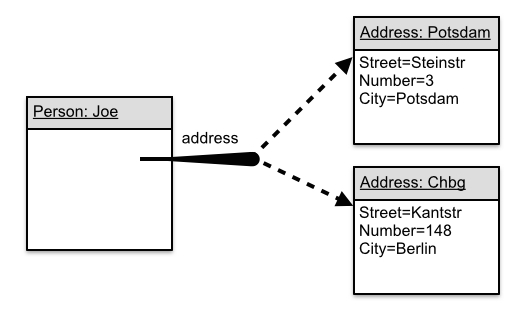
\includegraphics[width=0.5\textwidth]{figures/versionAwareReference.png}
    \caption{A Person object with two versions for its address.}
    \label{fig:VersionAwareReference}
\end{figure}

To resolve a path of an object graph as it was at a particular moment..., versions of objects are created and resolved in a coordinated way.
For this, the version-aware references have access to information on which version is currently the one that should be resolved to.
This can, for example, be a global version identifier that corresponds to information stored for each version of a version-aware reference, as shown in Figure~\ref{fig:MoreVersionAwareReferences}.
This example shows a slightly more comprehensive graph that might result from preserving specific versions while changing particular objects.
We have an initial version, \emph{v1}.
In this, a \emph{Company} object is created and that refers to a \emph{CEO} object using a version-aware reference.
The CEO in turn has an address, also referred to via a version-aware reference.
Next, we preserve this version and then, in version \emph{v2}, the same CEO moves to Berlin and, thus, his address gets changed.
Therefore, the version-aware reference to the address of the first CEO knows two different versions of the same address object.
Finally, to reach the situation shown in Figure~\ref{fig:MoreVersionAwareReferences}, we preserve the second version and change the company's CEO in version \emph{v3}.
We can also see that the new CEO also has its own address.
Now, given the knowledge that \emph{v3} is preceded by \emph{v2} and that by \emph{v1}, the version-aware references can resolve to three different development states the runtime was in.
When, for example, changing the CEO turns out to be a mistake, we can re-establish \emph{v2} and with it the old CEO with its address in Berlin as head of the company.
This way, when version-aware references are used consistently for all object relations in a programming runtime, the state of the entire runtime can be set to particular preserved versions.

\begin{figure}[h]
    \centering
    \includegraphics[width=\textwidth]{figures/MultipleVersionAwareReferences.png}
    \caption{Three versions visible in the version-aware references of a simple object graph.}
    \label{fig:MoreVersionAwareReferences}
\end{figure}

\todo{add code for the path through the object graph}
\todo{add version info (context info) to figures, where necessary}

\todo{add a Figure that shows the three versions of the company object graph separately and incorporate it into the text..}

Which states of the runtime get preserved is not inherent to our approach, but can be different for different use cases. % but also say that versions are created at specific times, specific state preserved (not all situations are recoverable)
Programmers could explicitly preserve versions or the programming system could do this implicitly.
When the programming system is resposible, each manipulating action of a programmer could, for example, yield a new version of the runtime, so programmers can reason about their concrete steps when undoing changes.
Actions that yield new versions could include directly manipulating attributes and composition of graphical elements, editing source code, evaluating do-its, and, for example, clicking buttons of an application.
This way, programmers could also always undo every actions, regardless of whether the action was intended as mere exploration and, thus, the current state protected by a version or whether the action turned out to be inappropriate more unexpectedly.
Using user actions as granularity allows developers to undo and redo the changes associated with specific and rememberable actions.



% transparency of version-awareness / versions

Version-aware references behave transparently, just like a usual reference to the current version of the object would.
They are assigned to variables and get passed around, and, under usual circumstances, programmers do not have to be aware of them.
Firstly, programmers should not be required to adapt their programs to use version-aware references.
Instead version-aware references should be provided consistently by the programming system.
Secondly, there should be no direct references to particular versions of objects.
Programmers should not have to distinguish between version-aware references and direct references, while having both direct references to one particular version and a version-aware reference that always refers to current version could also introduce inconsistencies.


% design implications & rationale

The resulting histories can be fine-grained as for each version only changed objects need to be copied.
Further, creating many versions is not expected to interrupt the programmers workflow as the execution costs of preserving a version is spread: Instead of copying all objects the moment a version should be preserved, objects are only copied when and in the moment they are subsequentely changed.
In general, the approach aims to distribute the cost for object versioning: besides incrementally saving a version, switching the active version is also not interruptive as the version-aware references resolve to versions dynamically and all versions reside as objects in application memory.


This version-aware references allow to change versions without stopping the system.
For this, the version-aware references resolve dynamically to particular versions based on context information.
Only this context information has to be changed to have all references resolve to another version, without updating any of the version-aware references.
Preserving a new version of the runtime also happens incrementally.
Instead of saving versions of all objects that make up the runtime, when the development state is to be preserved, new versions of objects can be created only when objects subsequentely change.
Before such writes the previous object states continue to reflect the current state and can, thus, be read for following versions until written.
This way, as \emph{objects} are copied on writes, versioning happens automatically on the granularity of objects.





\section{Using Proxies for Version-aware References} \label{sec:APPROACH:2}

% TODO STRUCTURE TODO

% what proxies do / how proxies are used as references/version-aware references

% source transformations to have proxies be used consistently
% garbage collection of proxies and versions

% rationale for using proxies:
% (as opposed to providing alternative references on virtual machine-level: language-level solution as there are many different engines used for executing JavaScript (which would all require implementations of version-aware references to have Lively with recovery support for all users. also implementation in JavaScript is easier (especially for a first prototype) and does not have to go through any formal review or standardization process, which language features added to JS engines usually do))


For a concrete solution for the Lively Kernel, we propose to use proxies for version-aware references.
These versioning proxies manage the different versions of an object and can delegate object access to one of these.
The references that usually refer to objects then need to refer to the proxies for these objects instead. 
This is accomplished by returning proxies directly when an object is created.
For this, we transform sources to proxy object literals and constructor functions.
Proxies for functions then return objects always proxied when used as constructors or otherwise to create new objects.
When these proxy-based version-aware references can know the versions of an object and are used consistently to access mutable objects, the proxies only need to know which versions to choose at a given moment and when to copy current versions to preserve particular runtime states.
For this, the runtime is enhanced with a global version identifier representing the current version, which the proxies use to annotate newly proxied objects or new versions of objects with and also to choose the correspondingly annotated versions when accessing proxies.
This then is enough to provide a simple undo/redo for Lively.


The proxies required for our solution are virtual-object proxies, proxies that can intercept and response arbitrarily on access.
Such proxies are usually not associated with a particular object or, in our case, version of an object.
When such a fully virtual object proxy is created for an exisiting or new object, the object needs to be just one among potentially many different versions of an object that the proxy might need to forward access to.
The proxies need to be able to intercept and arbitrarily handle all kinds of access transparently.
In fact, the proxies need to fulfill at least three responsibilities:
\begin{enumerate}
    \item They need to know which versions are available for a particular object.
    \item They need to choose one particular version among all available dynamically using context information.
    \item They need to delegate object access transparently to a chosen version.
\end{enumerate}


% TODO: incorporate how version-aware references get resolved into the above sections

% 
% Proxies hold multiple versions of an object.
% They can transparently delegate access to one particular among many versions.
% They are also referred to consistently instead of the object.
% This allows to have and use particular versions of particular objects.
% However, to enable programmers to undo and redo arbitrary changes to the entire development state, our solution needs to preserve and choose versions of all objects in a coordinated way and be able to establish particular versions of the entire runtime instead of just of single objects.
% Our solution to this is declaring versions of the runtime and, then, annotating versions of objects with the version of the runtime they are part of.
% 
% 
% \todo{continue here: write this subsection.. and figure out what details to explain here and which as part of the implementation...}
% 
% 
% global version information: linear: versions with predecessors and successors, maybe with a figure..
% 
% These information are used to decide to which particular versions of objects proxies are to delegate at any moment.
% Given which version of the runtime is currently active, the proxies can choose the corresponding version of the object.
% 
% 
% This way, the proxies transitively all delegate to objects that accurately represent the state of the entire runtime as it was at a particular moment---when the version of the runtime was last active.
% To preserve a development state, the version of the runtime just has to be changed.
% 
% 
% 
% 
% The version of the runtime can be global in JavaScript as JavaScript engines use only a single thread and cooperative scheduling.
% There is, therefore, no way to change which version of each object should be used while a path through an object graph is already partly resolved.




% TODO: subsubsection / paragraph on garbage collection

In our solution, we used the proxies also to hold all versions of the object they stand-in for.
This way, when the proxy is no longer reachable and, thus, eventually garbage collected, all versions of the objects are also collected.
For example, in the following code snippet, there would temporarily exist a version-aware reference---a proxy---connecting the \emph{Person} object to an \emph{Address} object, but the reference gets deleted before a version of the person is preserved:


\iffalse
\begin{verbatim}\fi
\begin{code}[lst:example]{}{float,numbers=left}
    var person = {name: "Lauritz"};
    \\ preserve first version
    person.currentAddress = {street: "Friedrichstrasse",
                         number: "112b",
                         city: "Berlin"};
    delete person.currentAddress;
    \\ preserve second version
\end{code}
\iffalse
\end{verbatim}\fi

That is, the address object is not required to re-establish either \emph{Version 1} or \emph{Version 2} and, thus, nothing should prevent the garbage collector from claiming the proxy for the address object and the address object itself.





% TODO: how to use these proxies to refer to mutable objects / subsubsection or paragraph

% \subsection{Proxies For All Mutable Objects}

% This ensures that references to proxies are used consistently instead of direct references to objects and that such proxies are used for every object.

When proxies are supposed to provide a kind of alternative references, ordinary references that usually point directly to an object now need to point to an object's proxy instead, which then can refer to one or multiple versions of the object.
To have all references refer to proxies instead of actual objects, proxies are created and returned for each new object when objects are created.
The only reference to the actual object---or, more precisely, the initial version of an object---remains inside the proxy, while the reference to the proxy gets passed around instead.
Therefore, all access goes through the proxy and the proxy forwards the access to a particular version of an object.
Also, all references that would usually point to the same object now point to the same proxy, so that proxies provide object identity.
Checks that would usually compare an object with other objects now compare a proxy with other proxies.

For this solution, all expressions that create new objects need to return proxies for those instead.

% TODO: move concrete steps to the implementation, state the following much more abstractly 

% TODO: when/wherever the following is expressed, the three categories should be three similarly named paragraphs after the initial introduction of the categories in the list

% In JavaScript, there are three different ways to create an object: 
% \begin{itemize}
%     \item evaluating literal expressions: e.g. \lstinline|{age: 12}|
%     \item applying constructor functions: e.g. \lstinline|new Person(12)|
%     \item calling specific built-in functions: e.g. \lstinline|Object.create(prototype, {age: 12})|
% \end{itemize}

% We use source transformations to wrap literal expressions consistently into a \emph{proxyFor()} function.
% That function takes an object as parameter and returns a proxy for it.
% Besides objects, arrays and functions are also mutable objects in JavaScript.
% Therefore, we wrap the literal forms of objects, arrays, and functions.
% For exampe, \lstinline{[aPerson, aCompany]} becomes \lstinline{proxyFor([aPerson, aCompany])}.
% 
% In JavaScript, all functions can be constructors and create new objects when called with the \emph{new} operator.
% Functions expressed as function literals already get proxied with the previous source transformations and the proxies we use for version-aware references intercept different object access differently, so proxies for functions can have a specific constructor-behavior that always returns proxies for newly created objects.
% 
% For the functions that create new objects but are built-in and, thus, are not created from literal form, the transformation of literals and proxy behavior is not enough.
% One category of such built-in functions are built-in constructors.
% For example, the built-in data types like objects and arrays can be created by evaluating \lstinline{new Object()} and \lstinline{new Array()}, but also by evaluating just \lstinline{Object()} or \lstinline{Array()}.
% We transform these built-in constructor functions explicity, wrapping each into the proxying function, and also specify the proxies' apply-behavior to also always return proxies.
% Besides these built-in constructors, there are also very specific built-in functions, that we transform separately to specific alternatives.
% One example for such functions is the global \lstinline{eval()} function.
% While the return value of that function also potentially needs to be a reference to a proxy instead of an ordinary object, eval takes arbitrary code which might express an arbitrary object structure and which might, therefore, require multiple references to go through proxies.
% Therefore, in the specific case of eval, we proxy eval's result but in addition also pass the string argument of \lstinline{eval()} through the source transformations before actually providing it for evaluation.



Proxies allow a language-level implementation of alternative references in JavaScript:
Without requiring adaptions to the virtual execution engines, proxies can be inserted to stand-in for objects---so references that usually point directly to objects point to proxies instead---and these proxies can provide versioning information and behavior.
These proxies are, thus, an alternative to using ordinary references to directly refer to objects.
That is, some objects can, potentially, still be referred to directly, while objects that should be versioned should be accessed only though proxies.
In our solution for Lively, nearly all objects are only accessed through proxies, except for some particular \emph{root objects} that are not required to be versioned but potentially do refer to other objects via version-aware references.

